\chapter{Modelagem do sistema computacional}\label{chap:software}

% Neste capítulo serão apresentados os aspectos para o desenvolvimento da ferramenta, como os pré-requisitos, escolhas das ferramentas, decisões de modelagem, e as práticas adotadas no processo.

O levantamento dos requisitos de um sistema é o elemento que fornece elementos que dever nortear uma série de decisões a serem tomadas no seu desenvolvimento. A ferramenta proposta visa agilizar o fluxo de trabalho do profissional que realiza análises de vida a fadiga, ou seja, propõem-se o seguinte fluxo padrão:

\begin{figure}[!ht]
    \centering
    \caption{Fluxo de operação proposto para a ferramenta.}\label{fig:workflow}
    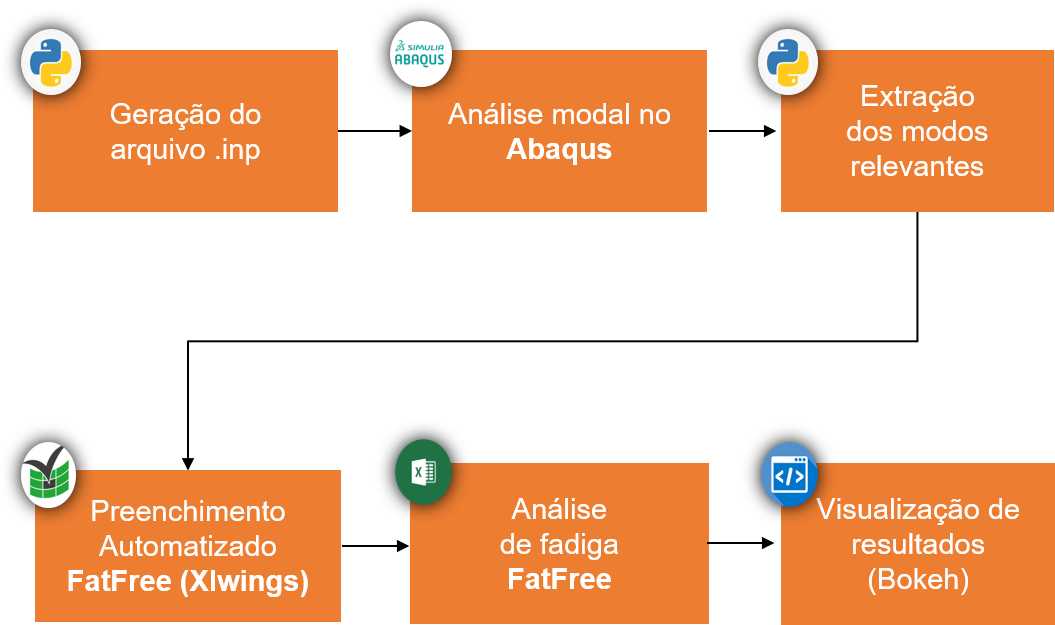
\includegraphics[width=0.7\textwidth]{imagens/workflow}
\end{figure}

De forma mais detalhada, a ferramente deve:

\begin{enumerate}
    \item A partir de um arquivo de entrada com informações do modelo, criar arquivos de entrada para o ABAQUS (\texttt{.inp}) que simulem todo o processo de simulação do comportamento do duto apresentado (\autoref{chap:assentamento}).
    \item Submeter o arquivo gerado para análise no ABAQUS.\@
    \item Processar os arquivos de saída do ABAQUS (\texttt{.odb}) extraindo os informações relevantes como a configuração deformada, modos de vibração, etc., gerando arquivos em outros formatos de fácil leitura para pós-processamento, tanto por esta ferramenta, quando por outro \textit{softwares}.
    \item Pós-processar as as informações gerando gráficos e relatórios relevantes para as tomadas de decisão do usuário quanto ao projeto. Esse é o requisito mais crítico, uma vez que é fundamental o entendimento sobre a análise de tudo em vão livre. Entre as tarefas que fazem parte deste itém está a automação da escolha dos modos de vibração ativos e relevantes e para cada vão de interesse -- a qual deve ser norteada pelos aspectos discutidos na~\autoref{sec:multimode} -- e a manipulação da FatFree\footnote{Planilha Microsoft Office Excel desenvolvida pela DNV-GL focada no cálculo de vida a fadiga de dutos submarinos.}.
    \item Apresentar os resultados finais na forma de gráficos e relatórios.
\end{enumerate}

\section{Computação científica}

Embora o uso e desenvolvimento de softwares de cunho científico seja uma atividade extremamente importante para pesquisadores, nem sempre são observadas boas práticas são observadas no seu desenvolvimento~\cite{Hannay2009}.
\citeonline{Wilson2014} apresenta um conjunto de boas práticas a serem adotadas no desenvolvimento desse tipo de. A seguir é apresentado o resumo do autor sobre essas práticas:

\vspace{0.5cm}
\begin{tcolorbox}[breakable, enhanced]

\textbf{Boas práticas para computação científica}

\begin{enumerate}
\item \textbf{Escreva programas para pessoas, não para computadores.}
    \begin{enumerate}
        \item Um programa não deve exigir que seus leitores mantenham mais de um punhado de fatos na memória de uma só vez.
        \item Torne os nomes consistentes, distintos e significativos.
        \item Tornar consistente o estilo e a formatação do código.
    \end{enumerate}

\item \textbf{Deixe o computador fazer o trabalho.}
    \begin{enumerate}
        \item Faça o computador repetir tarefas.
        \item Salve comandos recentes em um arquivo para reutilização.
        \item Use uma ferramenta de construção para automatizar fluxos de trabalho.
    \end{enumerate}

\item \textbf{Faça alterações incrementais.}
    \begin{enumerate}
        \item Trabalhe em pequenos passos com feedback frequente e correção de rumo.
        \item Use um sistema de controle de versão.
        \item Coloque tudo o que foi criado manualmente no controle de versão.
    \end{enumerate}

\item \textbf{Não se repita (ou repita outros).}
    \begin{enumerate}
        \item Todos os dados devem ter uma única representação oficial no sistema.
        \item Modularize o código em vez de copiar e colar.
        \item Reutilize o código em vez de reescrevê-lo.
    \end{enumerate}

\item \textbf{Planeje erros.}
    \begin{enumerate}
        \item Adicione asserções aos programas para verificar seu funcionamento.
        \item Use uma biblioteca de testes unitários pronta para uso.
        \item Transforme erros em casos de teste.
        \item Use um depurador simbólico.
    \end{enumerate}

\item \textbf{Otimize o software somente depois que ele funcionar corretamente.}
    \begin{enumerate}
        \item Use um \textit{profiler} para identificar gargalos.
        \item Escreva o código na linguagem de nível mais alto possível.
    \end{enumerate}

\item \textbf{Documente design e finalidade, não a mecânica.}
    \begin{enumerate}
        \item Documente interfaces e razões, não implementações.
        \item Refatore o código, em vez de explicar como ele funciona.
        \item Incorpore a documentação do software no próprio software.
    \end{enumerate}

\item \textbf{Colabore.}
    \begin{enumerate}
        \item Use revisões de código de pré-\textit{merge}.
        \item Use a programação em pares ao interar alguém novo e ao lidar com problemas particularmente difíceis.
        \item Use uma ferramenta de acompanhamento de problemas.
    \end{enumerate}
\end{enumerate}
\end{tcolorbox}


\section{Implementação}


Em observância a estas práticas, algumas decisões relativas ao desenvolvimento da ferramenta foram tomadas, e serão apresentadas a seguir.


\subsection{Linguagem de programação}

A linguagem adotada será Python\footnote{https://www.python.org}. Além de ser uma linguagem interpretada de alto nível Orientada a Objeto -- que permite um alto índice de reaproveitamento de código -- e da sintaxe simples, \citeonline{rao2018} apresenta algumas das principais vantagens que destaca a linguagem para este tipo de aplicação:

\begin{itemize}
    \item Disponibilidade de bibliotecas para aplicações cientificas contemplando manipulação de matrizes (Numpy), funções matemáticas (SciPy), manipulação de dados em forma tabular (Pandas), criação de gráficos interativos (Matplotlib e Bokeh);
    
    \begin{figure}[!ht]
        \centering
        \caption{Amostra das principais bibliotecas científicas em Python.}\label{fig:python_ecosystem}
        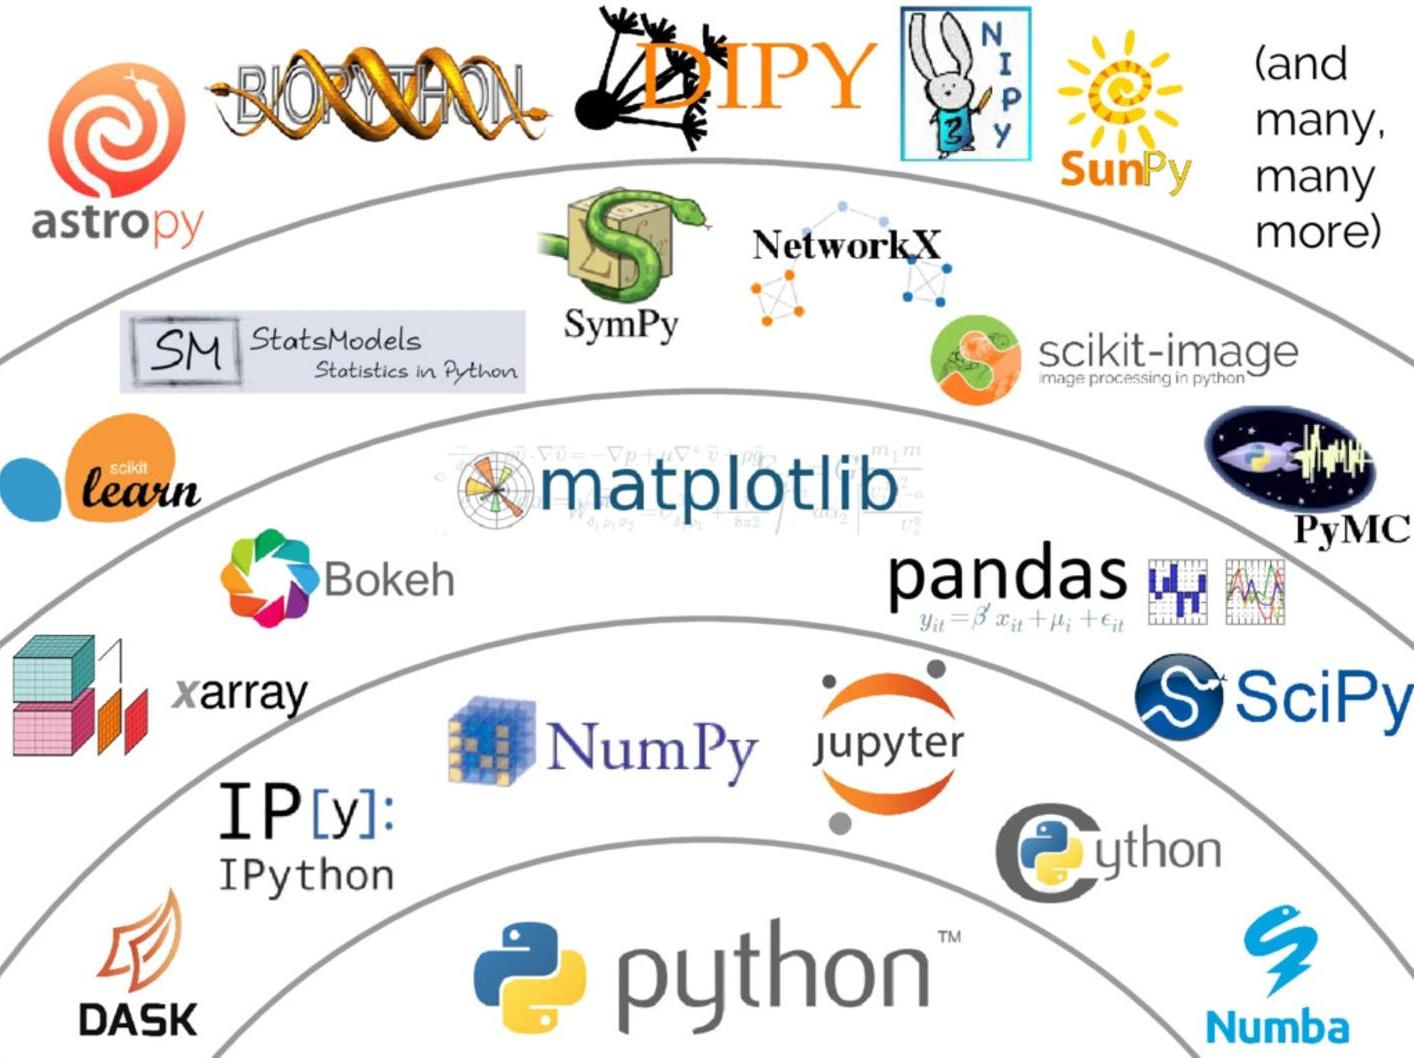
\includegraphics[width=0.6\textwidth]{imagens/python_ecosystem}
        \fonte{\citeonline{DataCamp2017}}
    \end{figure}

    \item Suporte para automação de tarefas. Os recursos de \textit{script} internos do Python e vários pacotes têm um forte suporte à automação de tarefas. A automação de tarefas repetitivas e a realização do registro de dados são fáceis e requerem pouco esforço.
    
    \item Pacotes Python como Django e Flask tornam possível desenvolver e usar o Python como uma API\footnote{Na programação de computadores, uma Interface de Programação de Aplicativos (\textit{Application Programming Interface} -- API) é um conjunto de definições de sub-rotinas e ferramentas para a criação de software. Em termos gerais, é um conjunto de métodos de comunicação claramente definidos entre vários componentes.} com um \textit{front-end} da web. Essa funcionalidade é particularmente útil ao usar uma infraestrutura baseada em nuvem como plataforma para acessar \textit{back-ends} de computação de alto desempenho (HPC).
\end{itemize}


\subsection{Estrutura de módulos e classes}

Para implementação do fluxo de trabalho proposto para a ferramenta, prevê-se a implementações de módulos para lidar com cada contexto específico. São eles:

\begin{itemize}
    \item \texttt{model\_generator}: módulo principal responsável orquestrar o fluxo de trabalho da ferramenta desde o processamento dos dados de entrada, geração dos arquivos para o ABAQUS e os pós-processamentos.
    
    \item \texttt{odb\_handler}: responsável por lidar com os arquivos de saída do ABAQUS (odb) e guardar os dados relevantes em arquivos com formatos de fácil manipulação (CSV, JSON, etc\ldots).
    
    \item \texttt{mode\_selector}: módulo responsável pela estratégia de seleção automática de modos de vibração para cada vão e manipulação dos dados associados vãos e seus respectivos modos.
    
    \item \texttt{dnv}: módulo que implementa os cálculos do modelos de resposta da \dnvf105 e manipula a planilha FatFree por meio da biblioteca xlwings.
    
    \item \texttt{plots}: módulo responsável pro agregar as funções de geração de gráficos dos resultados.
\end{itemize}

Já dentre as principais classes estão:

\begin{itemize}
    \item \texttt{Model}: classe que contém as informações do modelo do problema.
    A classe armazena todas as informações para construção dos arquivos \texttt{.inp}, isto é, dados de batimetria, material, geometria do duto, coeficientes de segurança, entre outros.
    A instanciação dessa classe deve ocorrer mediante o processamento de um arquivo principal de entrada com esses dados, possivelmente em formado JSON (\autoref{fig:json_sample}).

    \begin{figure}[!ht]
        \centering
        \caption{Aspecto de arquivo principal de entrada no formato JSON}\label{fig:json_sample}
        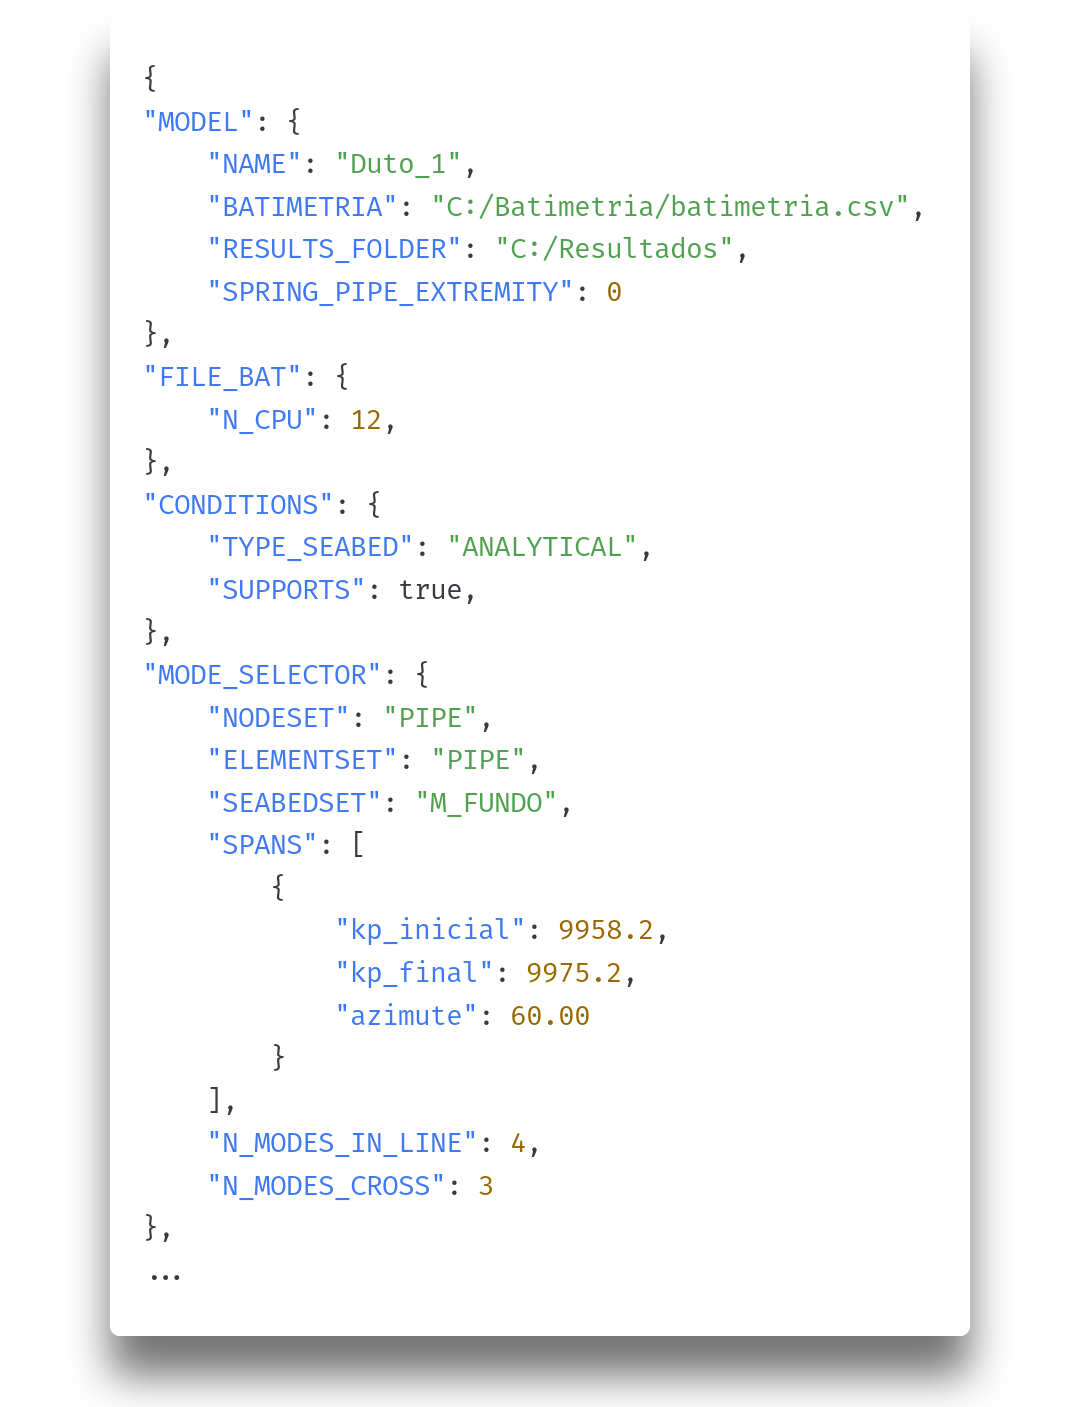
\includegraphics[width=0.5\textwidth]{imagens/json_sample}
        \fonte{Autor (2019)}
    \end{figure}
 
    \item \texttt{Inp}: lida com a escrita modularizada de arquivos de entrada  para o ABAQUS. A proposta é que se crie um arquivo principal que terá inclusão de outros arquivos acessórios que terão as informações específicas de cada aspecto da modelagem: batimetria, passos de carga, etc.
    
    \item \texttt{Span}: classe que representa um vão do duto. Dentre os métodos da classe estão os métodos responsáveis pela seleção dos modos de vibração.
    
    \item \texttt{ModeShape}: classe que representa um mode de vibração (\textit{mode shape}).
\end{itemize}

A \autoref{fig:UML} exibe um diagrama UML com esses módulos e classes, suas relações de pertencimento e dependência, e os principais métodos e atributos das classes.

\begin{figure}[!ht]
    \centering
    \caption{Diagrama UML dos módulos e classes.}\label{fig:UML}
    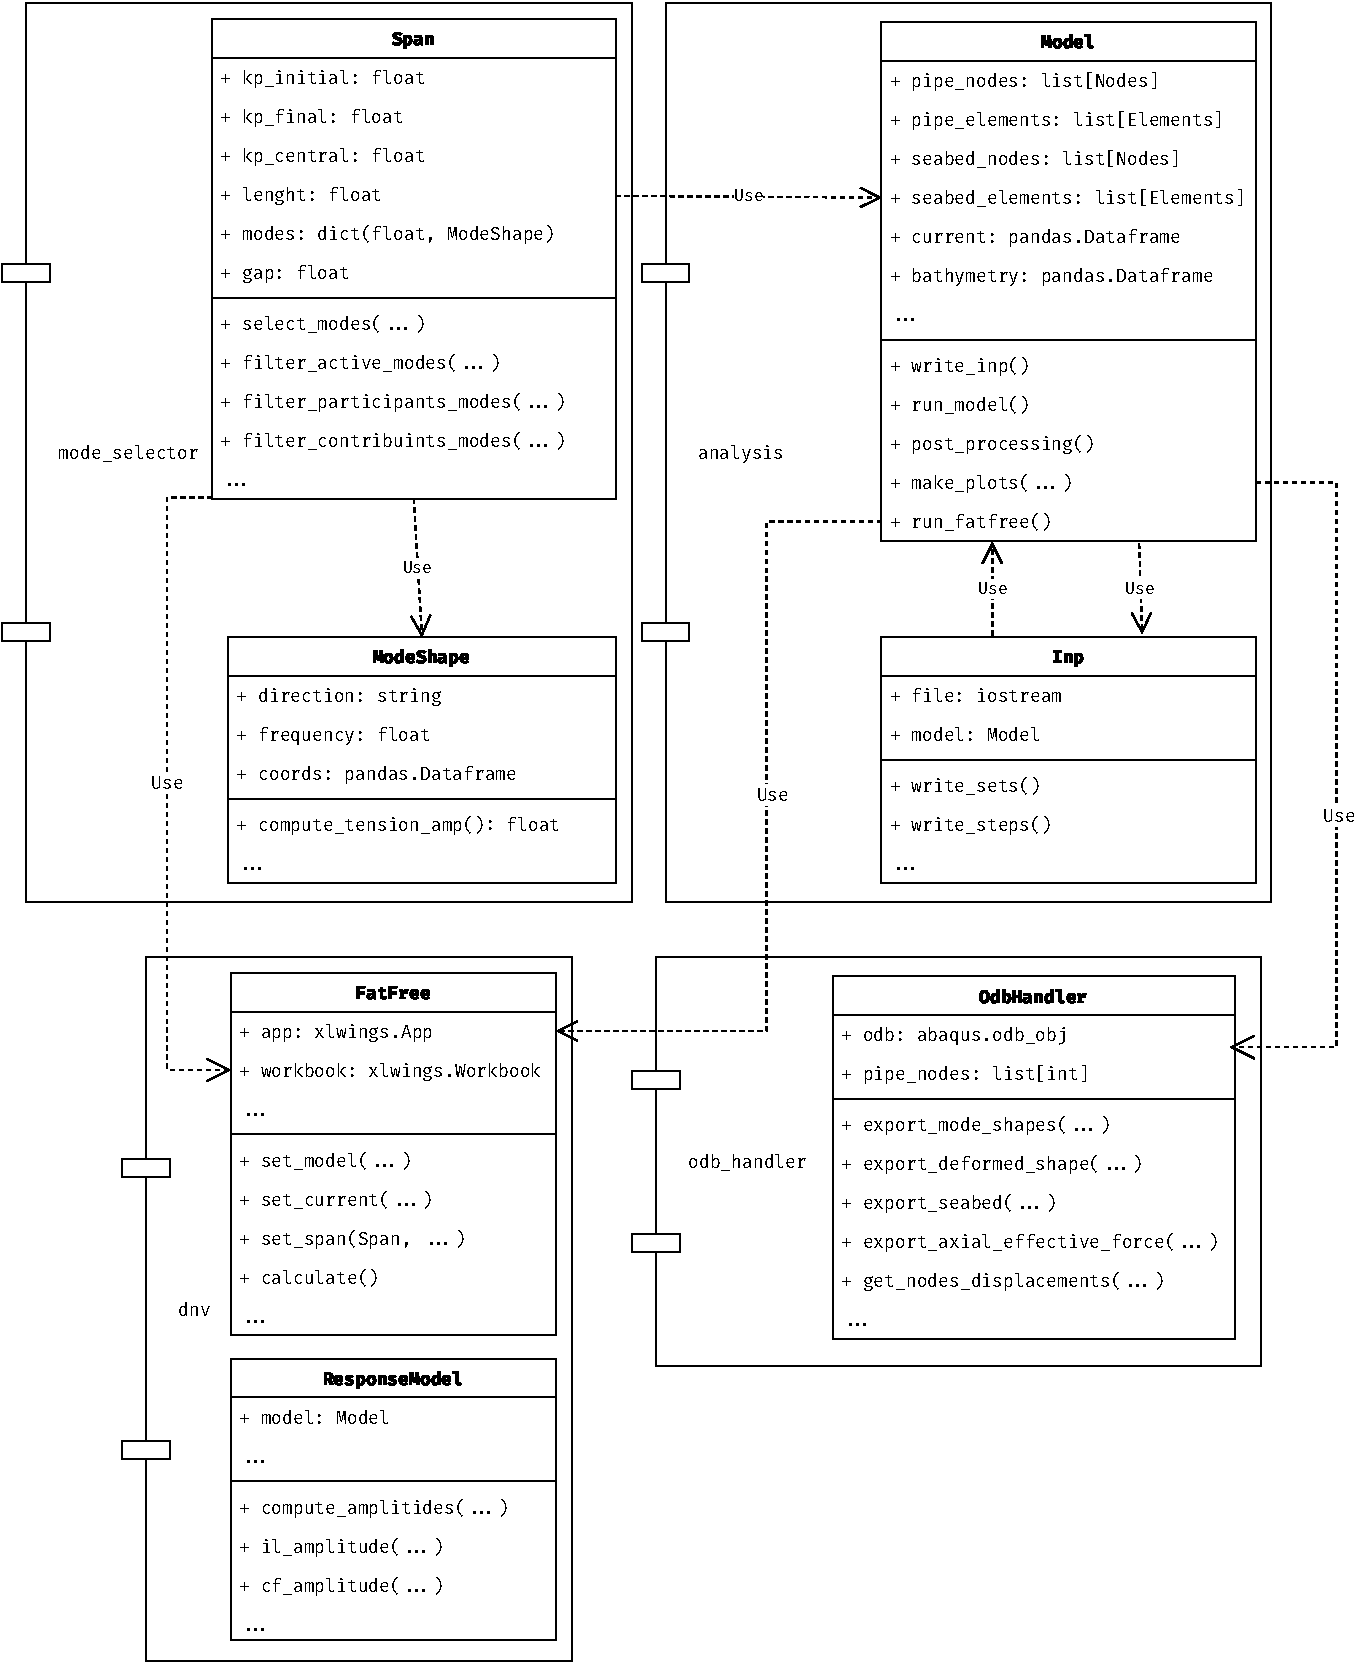
\includegraphics[width=0.95\textwidth]{imagens/UML}
    \fonte{Autor (2019)}
\end{figure}
